%                                                                 aa.dem
% AA vers. 8.2, LaTeX class for Astronomy & Astrophysics
% demonstration file
%                                                       (c) EDP Sciences
%-----------------------------------------------------------------------
%
%\documentclass[referee]{aa} % for a referee version
%\documentclass[onecolumn]{aa} % for a paper on 1 column  
%\documentclass[longauth]{aa} % for the long lists of affiliations 
%\documentclass[rnote]{aa} % for the research notes
%\documentclass[letter]{aa} % for the letters 
%\documentclass[bibyear]{aa} % if the references are not structured 
% according to the author-year natbib style

%
%\documentclass[twocolumn]{aastex61}

\documentclass[%
 aip,
 twocolumn,
 jmp,%
 amsmath,amssymb,
%preprint,%
 reprint,%
%author-year,%
%author-numerical,%
]{aastex61}
\usepackage{amsmath}
\usepackage{graphicx}% Include figure files
\usepackage{dcolumn}% Align table columns on decimal point
\usepackage{bm}% bold math
\usepackage{relsize}
\usepackage{subfiles}
%\usepackage{aastex}

%\usepackage[mathlines]{lineno}% Enable numbering of text and display math
%\linenumbers\relax % Commence numbering lines
\newcommand{\Msun}{$M_{\odot}$}
\begin{document}

%\preprint{AIP/123-QED}

\title[MEASURING DARK MATTER PROFILES NON-PARAMETRICALLY IN DWARF SPHEROIDALS]{MEASURING DARK MATTER PROFILES NON-PARAMETRICALLY IN DWARF SPHEROIDALS:
	AN APPLICATION TO LEO I}% Force line breaks with \\
\thanks{Footnote to title of article.}


\date{\today}% It is always \today, today,
             %  but any date may be explicitly specified

\begin{abstract}

We measure the central kinematics for the Milky Way dwarf spheroidal
galaxy Leo I. We find a rise in the velocity dispersion within the 
central $15"$.  Using axisymmetric, orbit-based models, we determine 
a black-hole mass of $2(\pm0.5)\times10^4$ \Msun\ can account for 
this rise.  At further radii, our kinematic data prefer a dynamical 
model which includes a dark halo; the radius where the enclosed dark
matter mass equals the mass of the baryons is 1'.  The inferred dark halo
from our models is smaller than previously published values ({\bf by how much}).
{\bf discuss simulations, and perhaps a concluding remark about no need for dark matter?
To address this discrepancy we run a suite of Monte Carlo simulations populating
fiber spectroscopy with the integrated light of stars from deep 
{\it Hubble Space Telescope} imaging.  We find a bias in the velocity dispersion
measurement towards higher values when only the brightest fibers are used.
We address this discrepancy with simplistic Monte Carlo simulations of 

At the distance of Leo I and with spectroscopic fibers of {\bf 3.2?}$"$
Our integral fiber unit observations of Leo I  dominated by single bright stars and fibers 
With extensive simulations to understand
potential biases in using individual velocities, we find that these
velocities need a correction applied that depends on the local stellar
density. We find consistent results between the integrated light
kinematics and the individual velocities when using results of the
simulations. Given these results for Leo I, we suggest other dwarf
spheroidal galaxy kinematics may suffer from a similar bias and should
be re-evaluated. The dynamical models can also accommodate a baryonic
component only in the galaxy, thereby removing the need for dark
matter from one of the most important cases that have been used to
signify the existence of dark matter.}

\end{abstract}

\pacs{Valid PACS appear here}% PACS, the Physics and Astronomy
                             % Classification Scheme.
\keywords{Suggested keywords}%Use showkeys class option if keyword
                              %display desired



\section{\label{sec:level1}}

\section{Introduction}

%Up to date, dwarf spheroidal galaxies are amongst the smallest scale dark matter dominated systems to which we have access. 
The study of the dwarf spheroidal galaxies within the local group provides a unique opportunity to characterize in detail the structure of dark matter subhaloes (e.g., Mateo et al. 1993; Walker et al. 2009; Łokas 2009). Unlike any other dark matter system, they are close enough to provide individual dynamical tracers that allow us to infer spatially detailed dark matter density profiles without significant baryonic disrupture. Like most dark matter systems, this inference is plagued with systematics and leaves room for competing explanations.



Which competing explanations?
What inferences?

- About stability (related to dynamical past). If high-eccentricity pericentric passage, dwarf could have experienced tidal heating due to tidal shock and even if this weren't the case, say the dwarf was in something close to a circular orbit, it could have subsequent/parallel tidal disrupture (The 'radius' of disrupture within the subhalo being hard to predict). Even if one were to look for rotational features studies have shown this could be misidentified or hardly present. This severely questions our ability to determine such a thing as a tidal radius (in itself an ill defined concept).

- About symmetry. We only have projected data. Yet our current models assume spherical symmetry due to need for tractability. The impact of this assumption is to be best of MY knowledge hard to understand (I guess one can get an idea from the CBE equation...)









%Several assumptions have traditionally entered our inferences when modelling dark matter substructures:

%- Assumptions of need (to make the problem tractable)
%- Assumptions 



Dwarf spheroidal galaxies 

detailed structure of subhaloes

are frequent choices for the
characterization of dark matter . As being systems that appear to be
significantly dark-matter dominated , they provide as pristine
representations for how dark matter interacts as we can find. The
earliest measurements of their kinematics (EdO and Taft, and others) show
a velocity dispersion that was much too large to explain with only their stellar content. Even though the earliest measurements used very few individual velocities for the
dispersion estimate (the first one only had three stars {reference}), subsequent
analysis still required dark matter {references}. Theoretical and numerical 
studies use dwarf spheroidal galaxies as lynchpins to infer the amount and
interaction rate of the elusive dark matter particle (many refs to look
up).

There has been a strong debate as to whether the shape of the central density
profile can be used to constrain the dark matter properties , or
whether baryonic physics dominate the density profile. The "core/cusp"
issues continues to be a difficult problem to solve . Most recent
reviews (find them) suggest that baryonic physics are the primary
explanation , without need to invoke self-interacting dark
matter. Furthermore, observational results are not decisive as to the
measure  of the central profile. Most studies (Mateo and co) show a
core to the central density , whereas the recent work of Jardel et
al. (2010?) show a cusp .

An interesting possibility is that dwarf spheroidal galaxies contain a
central black hole . Volonteri (2005?), Silk (2017?), Kormendy (2000?),
others have suggested that black hole formation may be a natural
consequence in these systems in the early universe. When extrapolated
to dwarf spheroidals, correlations between host galaxies and their
black holes suggest that these systems might expect to have black-hole
with masses of $1-10\times10^4$ \Msun. (Not sure how much we want to say
about gravitational wave detections at this point.)

Need paragraph on black hole limits in low-mass systems, and talk about BH-sigma relation.

Need paragraph on why Leo I and specifics about Leo I.




\subfile{DATA/DATA}

\subfile{KINEMATICS/KINEMATICS}


%In order to find VIRUS-W's individual fiber velocities and their corresponding errors we first use Cappellari \& Emsellem's (2004) penalized pixel fitting method (PPXF) to get an initial guess for the spectrum's redshift. PPXF works by fitting a linear combination of LOSVD convolved templates to the spectra and penalizing solutions that deviate from Gaussian for low S/N levels (I think this was like this...). For this purpose, we used a library of stellar templates priorly extracted with VIRUS-W using the procedure described in the above subsection. This templates had been redshifted to restframe using their own sky spectra as reference.

%As part of the byproducts of PPXF's fitting, one can get the best fitting linear combination of templates and the residuals from the fit. In order to measure the robustness of the linear combination of templates (i.e., to estimate the error), we characterize the residuals as a normal distribution and resample noise from such distribution. We then proceed to add this noise to the combined templates and create for each original spectrum 1000 artificial spectra with similar S/N. 
%Finally, we do a normalized cross-correlation of the set of artificially created spectra with the best matching template and get the mean and dispersion of this measurements. This two values serve as the radial velocity and error for each of our fiber spectra.

%In addition to our measurements, we also use a set of 328 published velocity measurements for Leo I (Mateo et al. 2008). 35 of those measurements fall within the angular coverage of our data set. Our new data set adds 477 measurements to those 35. Table one includes information on the two data sets.




\begin{deluxetable*}{lccccccccccc}
\tabletypesize{\scriptsize}
%\rotate
\tablecaption{Leo I Kinematic Datasets Properties\label{tab:proplog}}
\tablewidth{0pt}
\tablehead{
\colhead{} &\colhead{Bustamante et al.} & \colhead{Mateo et al.} }
\startdata
Instrument & VIRUS-W & HECTOCHELLE  \\
Number of Fibers & 477 & 328  \\
Angular Coverage & [2.57",1'32.84"] & [7.82",14'23.16"]  \\
Radial Velocity Range & [217.91,350.99] km/s & [260.10,311.10] km/s \\
Error Range & [0.38,97.74] km/s\tablenotemark{1} & [1.60,7.60] km/s \\
\enddata
\tablecomments{1: Within our sample, 224 fibers are below Mateo's maximum error. We keep the higher error measurements since their contribution gets properly weighted in our maximum likelihood estimation of Leo's LOSVD parameters. This is explained in further detail in the a following section.}
\end{deluxetable*}

\begin{figure}
\centering
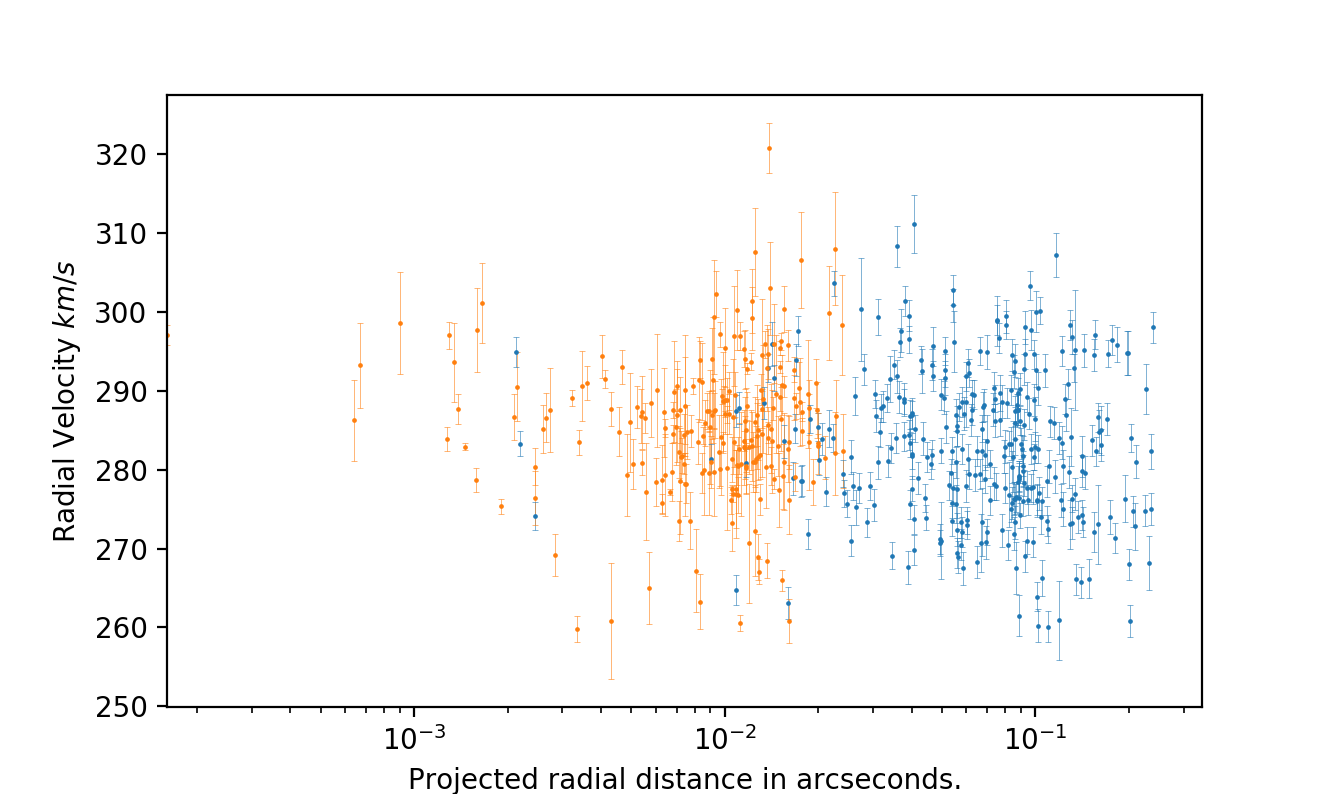
\includegraphics[width=0.5\textwidth]{LEOVELS.png}
\caption{Leo I data set (excluding points with errors higher than Mateo's dataset to ease visualization.)}       
\end{figure}
    
    
    
    

Given our instrumental resolution of ~8000 R, measurements of the dispersion that are below ~ 15 km/s are tricky specially with dealing with relatively low signal to noise levels. This made specially crucial to seek for confirmation using an alternative method

\subfile{CROWDING/CROWDING}
\subfile{LUMINOSITY/LUMINOSITY}



\section{DYNAMICAL MODELING}

We aim to determine the mass distribution of the galaxy that best fits both our spectroscopic and photometric data. The distribution, in general, can be characterized by the following equation:

\begin{equation}
\rho(r)=\frac{M_*}{L}\times\nu(r)+\rho_{DM}(r)+M_\bullet \delta(r)
\end{equation}

where:
\renewcommand\labelitemi{\tiny$\bullet$}
\begin{itemize}
	\item $\frac{M_*}{L}$: star mass-to-light ratio.
	\item $\nu(x)$: stellar luminosity density profile.
	\item $\rho_{DM}(r)$: dark matter density profile.
	\item $M_\bullet$: black hole mass.
\end{itemize}

Given a particular mass distribution, i.e., a particular set of the above variables, through Poisson's equations one can determine the corresponding gravitational potential. 






As inputs for the above equation one has, derived from data, the stellar luminosity density profile (which we described how to get in the above section). As free variables then, remain the dark matter density profile's parameters, the stellar mass to light ratio and the black hole's mass. Additional constraints, like axisymmetry around the equator, can (and have been, in the case of Leo I) established to further limit the potential's degrees of freedom.

Like so, a given set of derived and free parameters, under the assumption of the galaxy's relaxation time exceeding the age of the universe, allows one through the Collisionless Boltzmann Equation (CBE) to specify the likelihood of a large (ideally unbiased) set of allowed orbits occupying a given phase-space bin N number of times. Finally this can be compared with our kinematic data set and a specific set for such parameters in the above density equation gets selected for best fit. This, in broad terms, summarizes the principle behind our dynamical model, Schwarzschild's orbit-superposition method (Schwarzschild 1979), to better detail described in Gebhardt et al. (2000b), Thomas et al. (2004), and Siopis et al. (2009).

Specific to our case, was..... (Things like number of orbits, h3 and h4 priors, binning and dark matter profile type should go here...)


\bibliographystyle{unsrt}
\bibliography{leoI}
\end{document}


